\chapter{Planning System}\label{system}

In this chapter, take a look at how the GoDeliver\footnote{\url{https://godeliver.co/}} system works and the integration of the \gls{vrptw} \gls{ai} planner.

\section{GoDeliver System}

The GoDeliver system is consisted of multiple services, each responsible for a given subproblem of the delivery process. The core of the system is GoDeliver service, which implements all system APIs and performs the basic CRUD\footnote{Create, read, update and delete} operation on our NoSQL database. The database stores information about business, delivery orders, couriers, and delivery plans. In the Figure \ref{fig:godeliver-system} is visualized the simplified architecture of GoDeliver system, it is especially oriented to show how the planning process works.

\begin{figure}[ht]
    \centering
    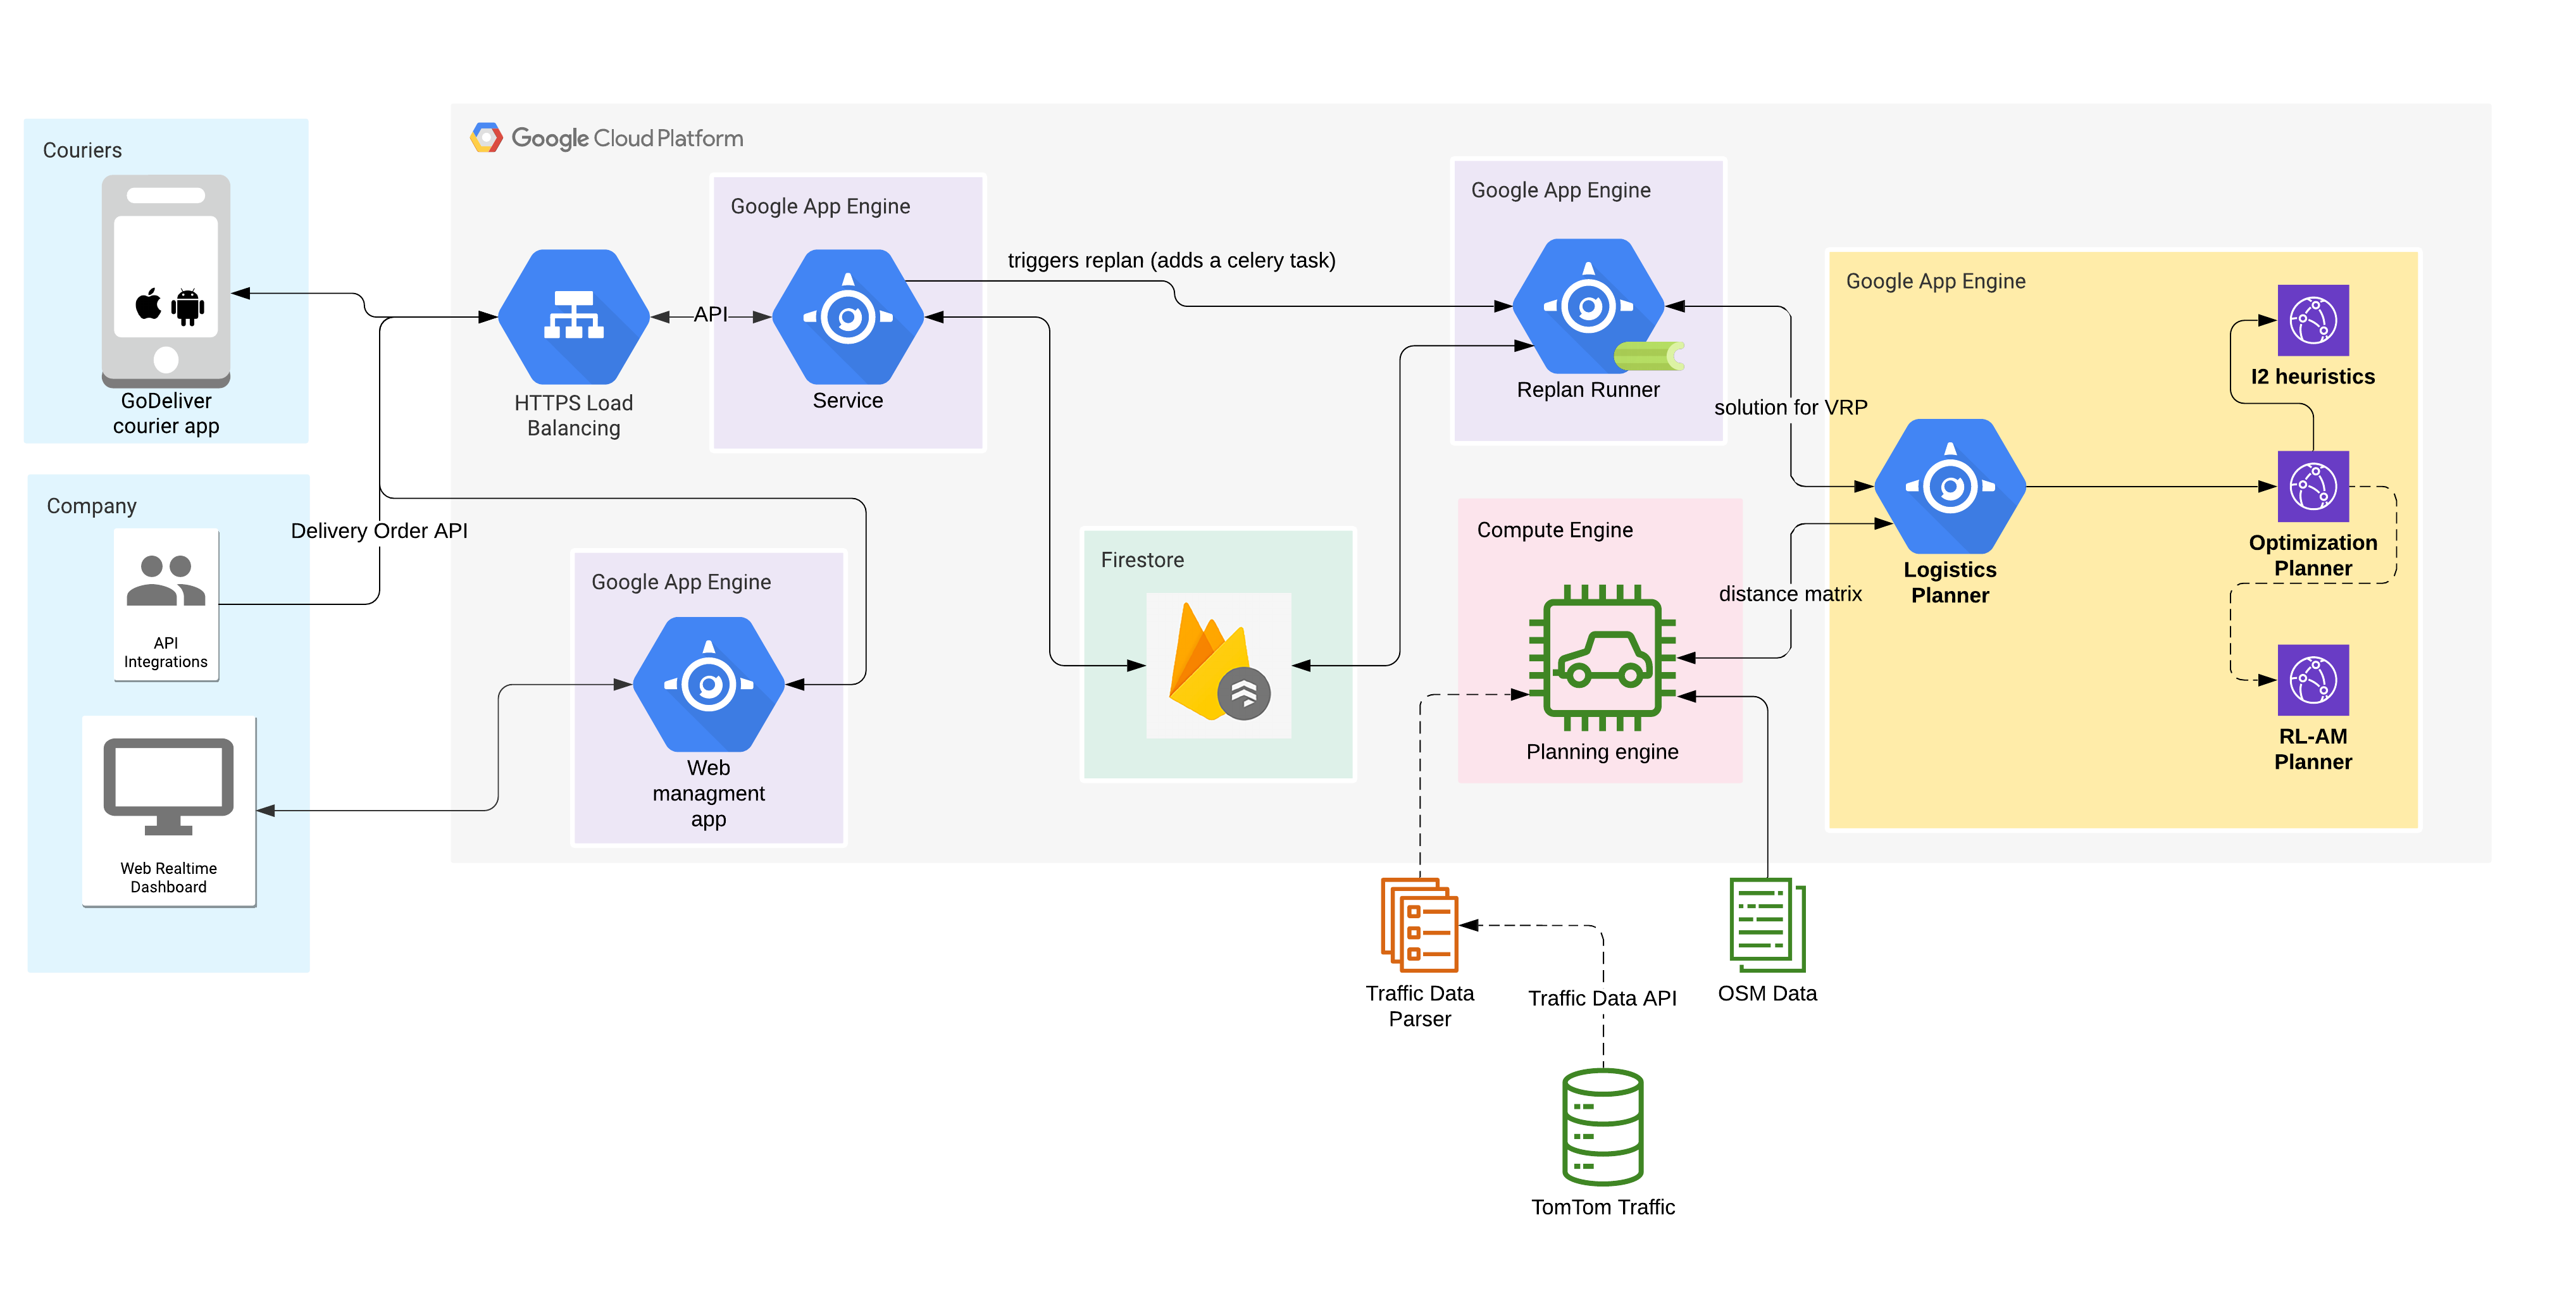
\includegraphics[width=1.0\textwidth]{resources/implementation/godeliver-system.png}
    \caption{GoDeliver System Architecture}
    \label{fig:godeliver-system}
\end{figure}

\subsection{Planning process}
The planning process is a complex operation which requires to work asynchronously because the planning of delivery orders is a time-consuming operation. The modern delivery planners have to support dynamic rescheduling and autonomously act upon the constantly changing environment.

The first part of the planning process is the creation of a delivery order, which is a request for delivery via API. The delivery order is saved in the database by GoDeliver Service with additional meta-data about the delivery state, etc. The database is monitored for a so-called \textit{trigger changes} which fires a replanning job via a distributed task queue Celery\footnote{\url{https://github.com/celery/celery}}. The \textit{trigger changes} are a list of actions such as creation of a new delivery order, changes in courier capacity, or a significant delay of delivery.

If such a replanning job is created, it is saved in Celery queue which is processed by GoDeliver Replanning Service \ref{fig:godeliver-system}. The replanning service loads a business configuration, delivery orders, and delivery plans from the database. It transforms the data into a generic structure which is accepted by our another service logistics planners that are solving the vehicle routing problem. The generic plan structure for the logistics planner freezes some delivery points which should not be considered by the planner since we do not want to change the current in-progress delivery points. This process is enabling us to perform the dynamic vehicle routing problem \ref{dynamic}.

Based on the business config, the desired vehicle routing solver is invoked via the logistics planner API. Usually, the planner takes the previous delivery plan and performs a heuristic algorithm like insertion heuristic which outputs an extended feasible plan. This plan is then improved by a local search algorithm to improve its cost function. Then the solution is processed by GoDeliver Replanning Service and saves the new delivery plans into the database.

\begin{figure}[ht]
    \centering
    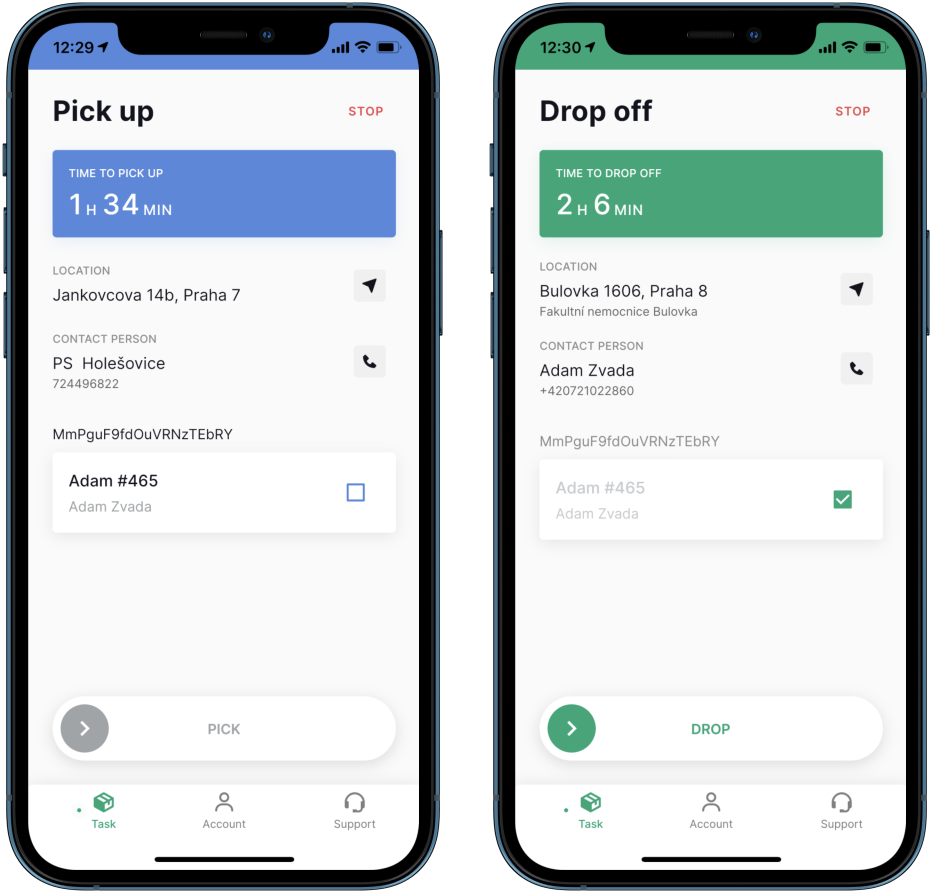
\includegraphics[width=0.75\textwidth]{resources/implementation/godeliver-app.png}
    \caption{GoDeliver Driver App}
    \label{fig:godeliver-app}
\end{figure}

In the future, the proposed \gls{vrptw} \gls{ai} planner will be used instead of insertion heuristics because we expect the \gls{ai} planner will outperform the insertion heuristics. The downside is that \gls{ai} planner is not able to leverage on the previous solution, which can lead to drastic changes in the solution structure of the delivery plan. However, this side effect is not a blocker since couriers only see one current delivery point from the delivery plan via GoDeliver mobile app \ref{fig:godeliver-app}.

\subsection{Planning Requirements}
The GoDeliver objective is to provide the most advanced and versatile urban logistics system. The logistics cases are always different for individual businesses and in order to cover them all we require a flexible but yet powerful planning system. For a new planner to be successfully used in the production environment, we have defined the planner requirements which have to be supported \ref{tab:vrptw-feature}. 

In the table \ref{tab:vrptw-feature}, we have summarized the supported features of our proposed \gls{vrptw} \gls{ai} It does not support features such as Pick and Deliver, predefined number of vehicles, and distance matrix. The Pick and Delivery is possible to support by extending the model to support a heterogeneous fleet based on this paper by J. Li et. al \cite{pick-deliver-ai} which extends the masking mechanism and \gls{rl} state and action to support the pick and deliver constraints. Distance matrix could be indirectly supported by applying multidimensional scaling \cite{multidimensional-scaling} to project the distance matrix into Euclidean space which is supported by the model. To define a fixed number of vehicles for a given \gls{vrptw} instance is surprisingly more complicated, but we propose that it can be achieved by implementing the support of multiagent reinforcement learning \cite{multiagent-rl} where each agent is one vehicle.

\begin{table}
     \centering
     \begin{tabular}{||c | c||} 
     \hline
     Feature & Is supported? \\ [0.5ex] 
     \hline\hline
     Time windows & \checkmark \\ 
     \hline
     Soft constraint & \checkmark \\
     \hline
     Distance matrix & indirectly\footnote{Multidimensional scaling \cite{multidimensional-scaling}} \\
     \hline
     Pick and Deliver & - \\
     \hline
     Demand Capacity & \checkmark \\ 
     \hline
     Balanced load across vehicles & \checkmark \\ 
     \hline
     Predefined number of vehicles & - \\ [1ex] 
    \hline
    \end{tabular}
    \caption{VRPTW AI support of planner requirements}
    \label{tab:vrptw-feature}
\end{table}

\section{Tech Stack - VRPTW via Optimization}

The planners based on optimization heuristics are implemented in programming languages Python\footnote{\url{https://python.org/}} and Go\footnote{\url{https://golang.org/}} and our implemented metaheuristic uses the optimization framework OR-Tools.

\section{Tech Stack - VRPTW via AI}

The \gls{vrptw} planner via \gls{ai} is implemented in the programming language Python which is the most favorite programming language for any \gls{ai}-related project \cite{stack-overflow}. Besides it is easy language to get start with, it has many amazing \gls{ai} and data libraries such as Pandas, Numpy, Tensorflow or PyTorch.

Production implementation of neural network is developed with the use of deep learning frameworks. TensorFlow\footnote{\url{https://pytorch.org/}} and PyTorch\footnote{\url{https://pytorch.org/}} are the two most popular frameworks. It is an important decision which deep learning framework to choose if you plan to develop a production ready \gls{ml} pipeline.

\begin{figure}[ht]
    \centering
    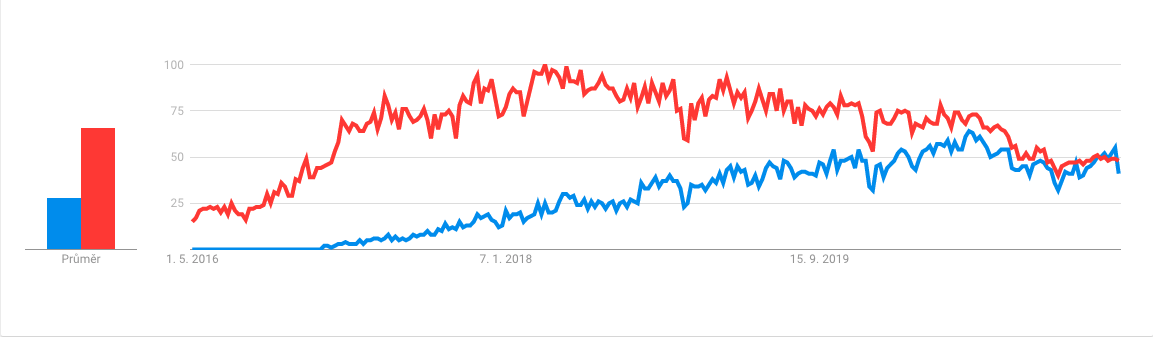
\includegraphics[width=1.0\textwidth]{resources/implementation/dp-framework-trend.png}
    \caption{Google Trend of PyTorch (blue) vs Tensorflow (red)}
    \label{fig:dp-framework-trend}
\end{figure}

The Google Trends graph \ref{fig:dp-framework-trend} shows how TensorFlow was more popular in the past, but lately they have similar amount of search results. However, the majority of the new research papers are implemented via PyTorch \cite{pytorch-data}. It is due to the fact that PyTorch has a great and intuitive API based on Numpy\footnote{\url{https://numpy.org/}} operations and it is even slightly faster than TensorFlow.

In this thesis, we have decided to use PyTorch as our main deep learning framework.


